\par{Listing \ref{more_work_kernel} its our attempt to give every 
    \emph{work item} more work, that way decreasing the effects of scheduling 
    and spawning overhead of \emph{work items} and \emph{work groups},
    this way the behaviour when cycles per \emph{work item} are increased can 
    be studied. This was achieved changing the dimension of the \emph{NDRange} 
    from 2 to 1 and making that every instance of a \emph{kernel} calculate the 
    results of one row of the resulting matrix, as it can be 
    seen in line \emph{10} of listing 4.}

\begin{figure}[!h]
    \centering
    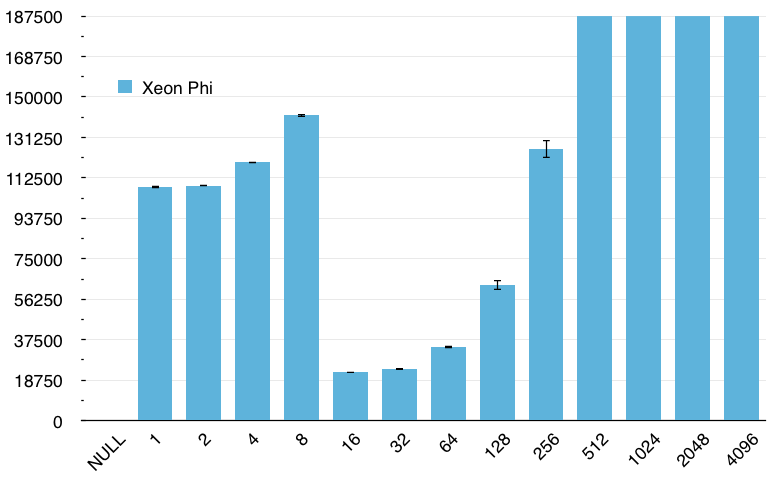
\includegraphics[width=0.49\textwidth]{figures/opt1_phi.png}
    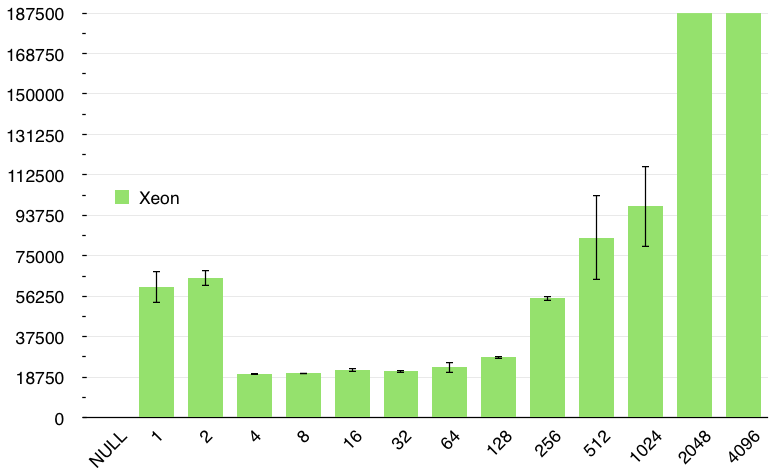
\includegraphics[width=0.49\textwidth]{figures/opt1_cpu.png}
    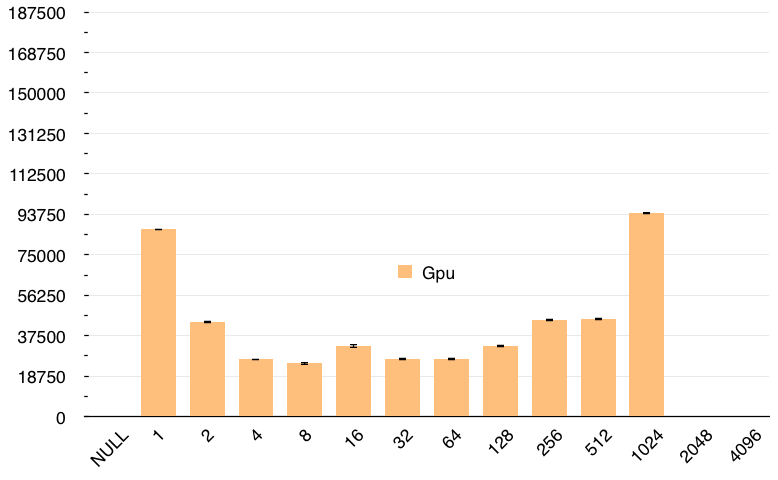
\includegraphics[width=0.49\textwidth]{figures/opt1_gpu.png}
    \caption{Results of matrix multiplication \emph{kernel} with more work per 
            \emph{work item} in different architectures.}
    \label{MoreWork}
\end{figure}

\par{Figure \ref{MoreWork} shows that in the case of the Xeon Phi co-processor 
    and the Xeon CPU, the effect of vectorization
    is the same that in the previous kernel(16 for the Xeon Phi and 4 for the 
    Xeon CPU), the other interesting effect in this
    case is the performance degradation after \emph{work group} dimension 32 
    on the Xeon Phi and after 128 on the Xeon
    CPU, clearly the Xeon Phi is more sensible to the decreasing number of 
    \emph{work groups} than the Xeon CPU, one of the 
    reasons for this is the number of \emph{computation units} available in 
    these 2 architectures, on the Xeon Phi is 236 and
    on the Xeon CPU is 40, as the number of \emph{work groups} decreases, 
    as it is shown on table \ref{tab:work_groups}, the amount
    of available parallelism that take advantage of the \emph{compute units} 
    available in these 2 architectures decreases as well.}

\par{The trend in figure \ref{MoreWork} for the GPU follows a different pattern
    than in the Xeon and Xeon Phi. After decreasing almost linearly for 
    \emph{work group} dimensions of 1 and 2, because of the increment of
    \emph{work items} executing in parallel in every SMX, the trend reach a 
    plateau. The execution time stop to decrease mainly because of the memory
    access pattern of the matrix A, which is completely strided, forcing the 
    system to access \emph{global memory} multiple times losing the performance
    gained by executing more \emph{work items} in parallel in a warp. For 
    \emph{work group} dimension of more than 512 you start to loose parallelism
    and take advantage of the 13 compute units in the GPU.}

\begin{table}[!h]
    \centering
    \begin{tabular}{| l | l | l | l |}
    \hline
    \emph{Work Group} Dimension & \#\emph{Work Groups} \\ \hline
    16 & 256 \\ \hline
    32 & 128 \\ \hline
    64 & 64 \\ \hline
    128 & 32 \\ \hline
    256 & 16 \\ \hline
    512 & 8 \\ \hline
    1024 & 4 \\ \hline
    2048 & 2 \\ \hline
    4096 & 1 \\ 
    \hline
    \end{tabular}
    \caption{\emph{Work group} dimension versus numbers of \emph{work groups}.}
    \label{tab:work_groups}
\end{table}

\par{In this case the most performant of the 3 architectures analized is the 
    Xeon as its shown on figure\ref{MoreWorkRes}. This could be explained by
    the small amount of parallelism needed to take advantage of the low number
    of compute units in the Xeon(40). Furthermore the execution of the kernel
    on the Xeon based on vectorization(2 modes) and the deeper cache hierarchy, 
    makes the Xeon not as sensible to the memory access pattern as the GPU.}

\begin{figure}[!h]
    \centering
    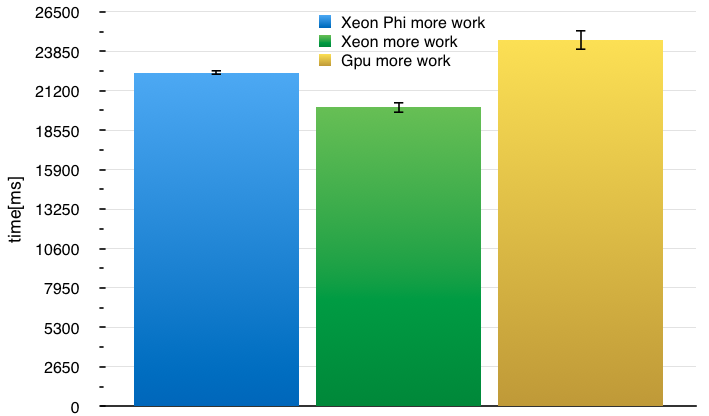
\includegraphics[width=0.49\textwidth]{figures/moreWorkRes.png}
    \caption{Comparison between the best cases of the more work \emph{kernel} in different devices.}
    \label{MoreWorkRes}
\end{figure}

\par{Figures \ref{gpu}, \ref{phi} and \ref{xeon} show that the 
    only device that obtained some performance improvements from this \emph{kernel}
    change was the Xeon. This is basically because the Xeon is the only architecture
    that does not need huge amount of parallelism like the GPU and the Xeon Phi.
    Intel recommends for the Xeon Phi to use at least 1000 \emph{work groups} and
    in the GPU the new \emph{kernel} affected the memory access pattern 
    changing it from coalesced to strided.





